\chapter{Design}
\justify

This chapter elaborates on the system design and architecture for the {\myprojectname} project.

\section{Project Overview}

The {\myprojectname} project aims to develop a robust system for collecting people's information for law enforcement purposes. The system design and architecture play a crucial role in ensuring the app's functionality, scalability, security, and ease of use.

\section{System Design}

The system design of the "{\myprojectname}" app encompasses several key components:

\begin{figure}
    \centering
    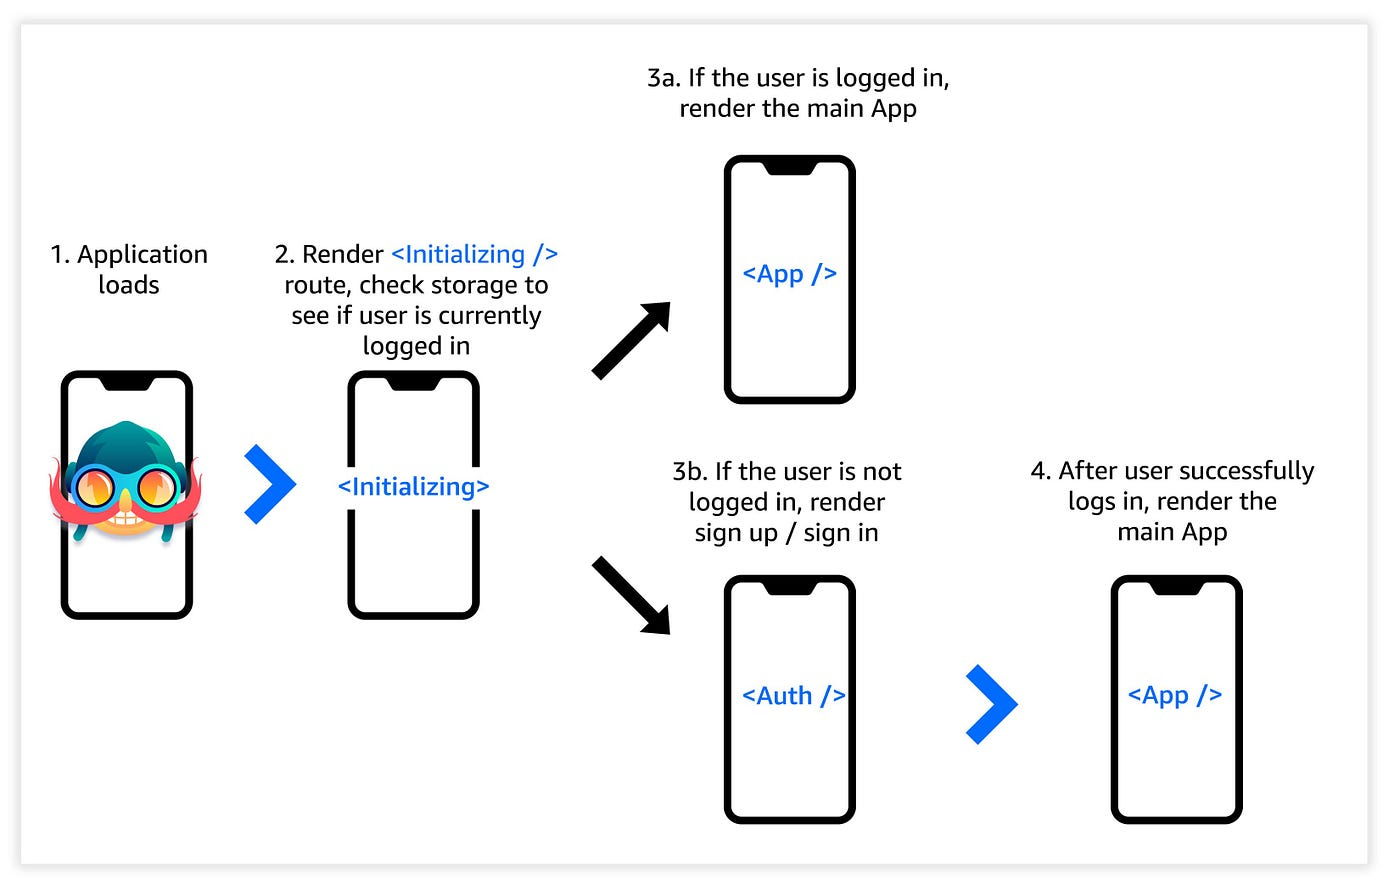
\includegraphics[width=1\linewidth]{Media//appFlow.jpg}
    \caption{App Flow}
    \label{fig:App Flow}
\end{figure}


\begin{enumerate}[label=\arabic*.]
    \item \textbf{User Interface (UI):} The UI design focuses on providing an intuitive and user-friendly experience for app users. It includes screens for data collection, settings, notifications, and law enforcement functionalities.
    
    \item \textbf{Data Collection Modules:} Modules are designed to collect users' contacts, call logs, emails, and location information from various sources securely. Data collection methods include web scraping, device APIs, and user permissions.
    
    \item \textbf{Data Storage:} A robust database management system is implemented to store collected data securely. The system ensures data integrity, accessibility, and compliance with legal and privacy standards.
    
    \item \textbf{Security Features:} The app incorporates encryption mechanisms, access controls, and authentication protocols to safeguard sensitive data, especially law enforcement-related information.

    \item \textbf{Scalability and Performance:} The architecture is designed to handle large volumes of data efficiently, ensuring scalability as user base and data collection grow. Performance optimizations are implemented for seamless app functionality.
    
    \item \textbf{Data Processing and Analysis:} Implementing data processing pipelines and analytical tools to cleanse, transform, and analyze collected data. This includes data normalization, pattern recognition, and predictive analytics to derive actionable insights for law enforcement agencies.
    
    \item \textbf{User Feedback Mechanisms:} Incorporating feedback mechanisms within the app to gather user input, suggestions, and reports on data accuracy or privacy concerns. Feedback loops help improve app functionalities and user experience iteratively.
    
    \item \textbf{Offline Data Access:} Designing the app to provide limited offline access to collected data, ensuring usability even in low connectivity or offline scenarios. Offline capabilities may include cached data access and synchronization when connectivity is restored.
    
    \item \textbf{Internationalization and Localization:} Adapting the app design and content for international users by incorporating multilingual support, localized content, and culturally sensitive UI/UX elements. This enhances user engagement and accessibility across diverse user demographics.
    
    \item \textbf{Accessibility Features:} Implementing accessibility features such as screen reader compatibility, text-to-speech functionality, high contrast modes, and adjustable font sizes to cater to users with disabilities and improve overall app inclusivity.
\end{enumerate}


\section{Architecture}

The architecture of the "{\myprojectname}" app follows a client-server model with the following components:

\begin{figure}
    \centering
    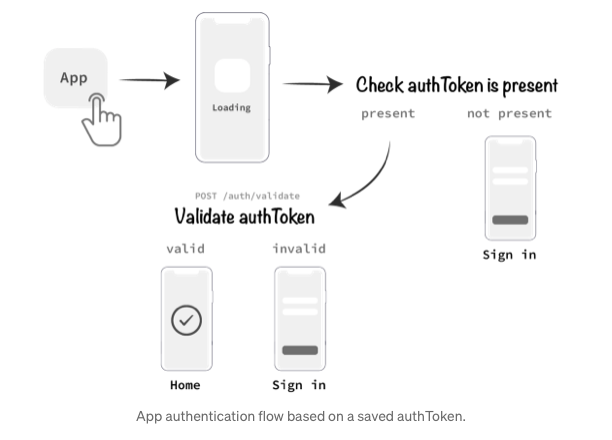
\includegraphics[width=0.9\linewidth]{Media//userLoginFlow.png}
    \caption{User Interface}
    \label{fig:User Interface}
\end{figure}

\begin{enumerate}[label=\arabic*.]

    \begin{figure}
        \centering
        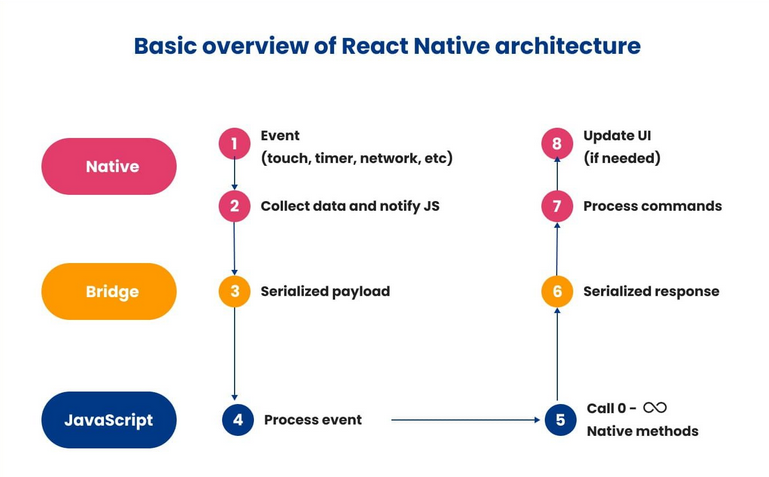
\includegraphics[width=1\linewidth]{Media/RNA.png}
        \caption{React Native Architecture}
        \label{fig:React Native Architecture}
    \end{figure}

    \item \textbf{Client Side:} The client-side comprises the mobile app interface accessible to users. It interacts with backend servers for data collection, storage, and retrieval.
    
    \item \textbf{Backend Servers:} Backend servers handle data processing, storage, and communication with external APIs and databases. They manage user requests, data synchronization, and law enforcement access.
    
    \item \textbf{Database:} A centralized database stores collected user data securely. It supports structured and unstructured data types, enabling efficient data querying and analysis.
    
    \item \textbf{API Layer:} An API layer facilitates communication between the client-side app and backend servers. It includes endpoints for data retrieval, updates, and law enforcement functionalities.
    
    \item \textbf{Security Infrastructure:} The architecture incorporates security measures such as HTTPS protocols, data encryption, firewalls, and intrusion detection systems to protect data integrity and privacy.
    
    \item \textbf{Cloud Integration:} Leveraging cloud computing services for scalable infrastructure, data storage, and computation resources. Cloud integration enables flexible deployment options, cost optimization, and improved scalability for handling varying user loads.

    \item \textbf{Data Backup and Recovery:} Implementing robust data backup and recovery mechanisms to ensure data resilience and continuity in case of system failures, disasters, or security incidents. This includes regular backups, disaster recovery plans, and data redundancy strategies.
    
    \item \textbf{Compliance Monitoring and Auditing:} Integrating compliance monitoring tools and audit trails to track data access, usage, and modifications. Compliance audits ensure adherence to regulatory requirements, industry standards, and internal policies.
    
    \item \textbf{Version Control and Release Management:} Implementing version control systems and robust release management practices to manage app updates, bug fixes, and feature enhancements. Versioning ensures consistency, compatibility, and traceability of app changes over time.
    
    \item \textbf{Performance Optimization:} Conducting performance profiling, load testing, and optimization efforts to enhance app responsiveness, scalability, and resource utilization. Performance optimizations may include code refactoring, caching strategies, and database indexing.
\end{enumerate}


\begin{figure}
    \centering
    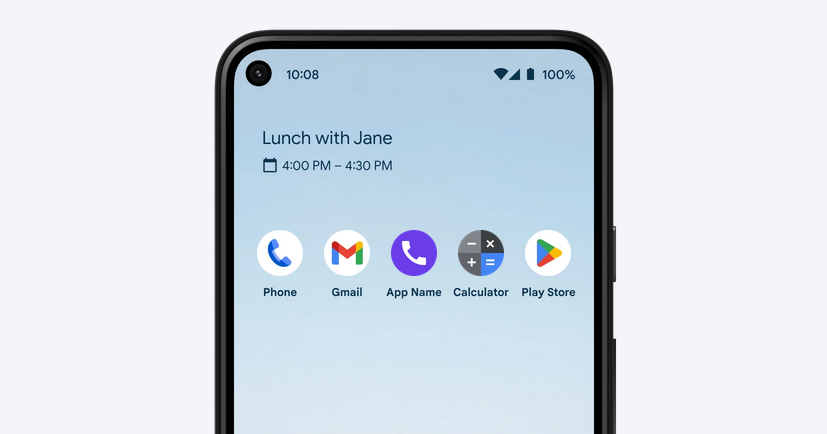
\includegraphics[width=1\linewidth]{Media//phone.png}
    \caption{App on phone}
    \label{fig:App on phone}
\end{figure}